\section{External Evidence and Its Limits}
\subsection{No new untouched-cohort confirmation}
No locally authenticated unused cohort was available under the optional final branch. Existing TopCoW/CAS analyses below remain analytical studies on public challenge training collections with the documented outcome-informed history, not newly untouched external neural confirmation.

\subsection{External Support, Scale, and Anatomical Checks}
These external MRA experiments are exploratory. The external MRA protocol was written before outcome calculation; it uses a different cohort from the historical brain T2 studies. All native images and labels remain unchanged. Complete cases, protocol versions, 250 source hashes, all mask choices and fixed-estimator benefit results are retained in the final reproducibility and evidence map.

\paragraph{Correcting bank-score provenance.}
The archived \texttt{target\_0.01} field denotes the target model's prediction mask, not ground truth. We independently recompute 84 mask/target/partner combinations from original predictions on the lexicographically first case in each cohort; maximum difference is $1.42\times10^{-14}$. Linear/Cubic are candidate members; the smaller denominator comes from neural-only target precomputation. The historical architecture studies's intervention masks remain ground-truth-derived. Across all 506 eligible model--case rows, acquired-input masks give median benefit correlations .863/.723, prediction masks .835/.710, and bank unions .805/.519 on fastMRI/NingXia. Acquired-mask partial medians given current error are $-.058/.425$. No mask is chosen based on these outcomes.

\begin{figure*}[t]
\centering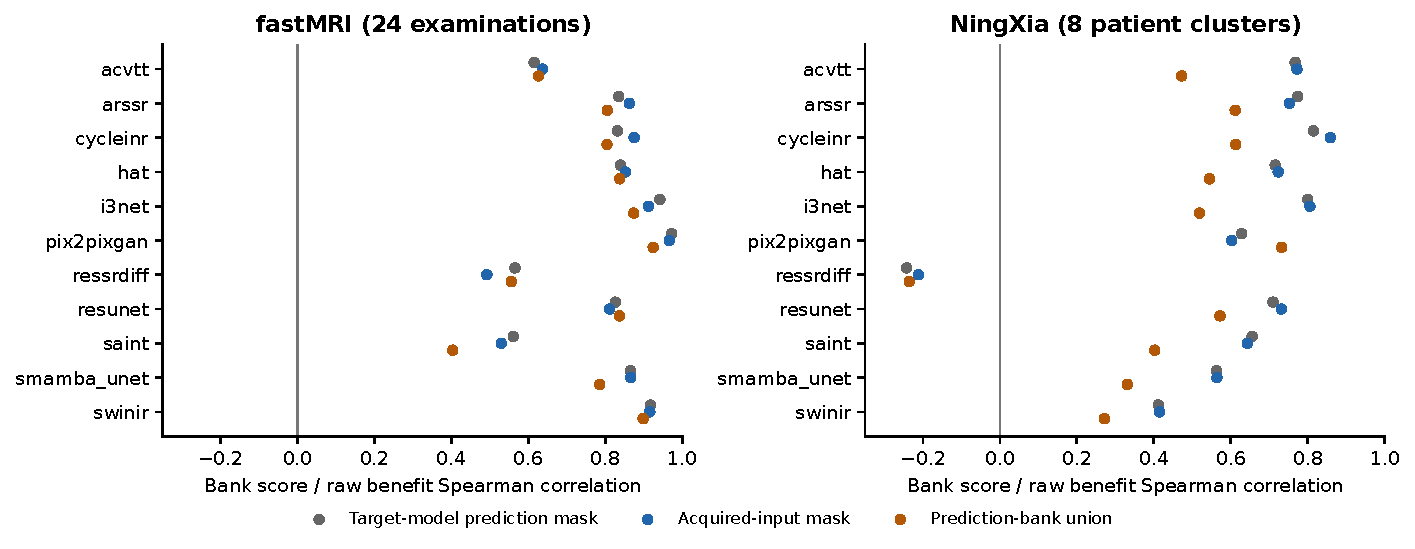
\includegraphics[width=.98\textwidth]{p14_bank_mask_sensitivity.pdf}
\caption{All 11 neural target models under three score-support contracts. Points are raw benefit correlations, not confidence limits. Linear/Cubic remain candidate members; neither was precomputed as a target model. All model-specific bootstrap intervals and paired mask differences are retained in the numerical record.}
\end{figure*}

\paragraph{Crossing score and endpoint units.}
For the 115 recovered IXI I3Net pairs, use the same acquired-anchor 1st--99th percentile range $r$ to form all four contracts: $(s,b)$, $(s/r,b)$, $(s,b/r)$, and $(s/r,b/r)$. Anchor-CV correlations are .843, $-.238$, $-.375$, and .539; adjacent MAE gives .845, $-.236$, $-.373$, and .551. Bootstrap count is 10,000 and seed 20260909. At 50\% selection, matched normalized Anchor-CV exceeds random by .000655 normalized MAE units [.000151,.001537], while the same score against raw benefit remains below random. Shared scaling can induce correlation, so unit consistency is not a causal or calibration guarantee.

\begin{figure*}[t]
\centering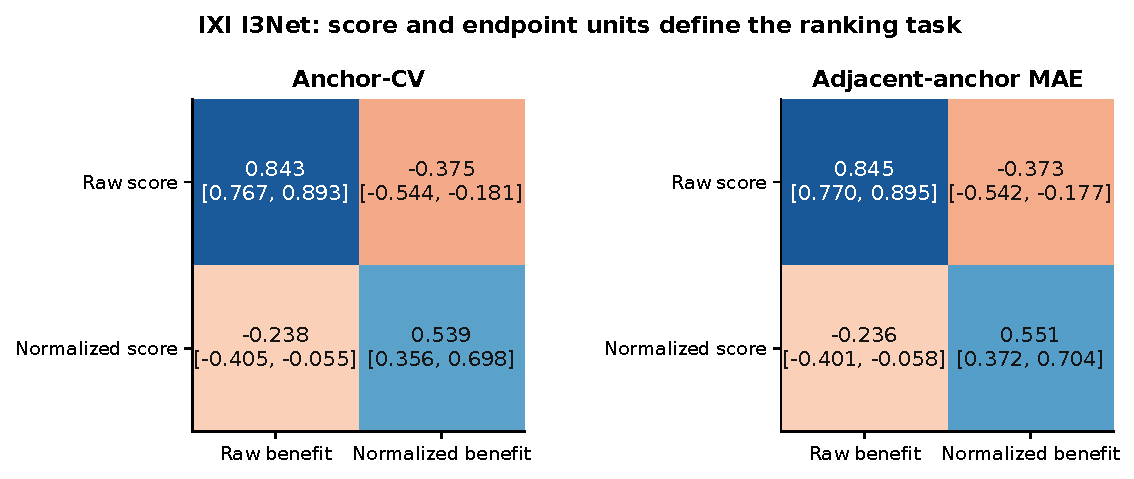
\includegraphics[width=.92\textwidth]{p14_scale_contract.pdf}
\caption{Score--endpoint unit contracts on IXI. Each cell gives Spearman correlation and an exploratory pointwise 95\% examination-bootstrap interval. Both favorable diagonal cells and adverse off-diagonal cells are reported.}
\end{figure*}

\paragraph{External MRA protocol.}
We use all 125 locally available annotated TopCoW MRA cases (public challenge training data, no fitting in this experiment), with 10779 eligible odd planes. L is linear interpolation; C is four-point Lagrange interpolation with no output clipping. For each phase, all four cubic anchors must lie inside the image; neither boundary duplication nor label-based plane selection is allowed. L$_0$--C$_0$ and C$_0$--L$_0$ are shared controls; their disjoint partners are C$_2$ and L$_2$. The input-support mask is the union of the two nearest acquired phase-0 anchor masks, each thresholded at 1\% of that anchor's maximum absolute intensity. The full-image and target-derived-mask alternatives are sensitivity contracts, not pooled replicas. Within each case, means are first taken within target residues 1 and 3, then the two residue means are equally weighted. Cases are the bootstrap units; 10,000 common draws are used. Local-gain simultaneous intervals use the maximum standardized deviation across the two estimator pairings within each mask. Other intervals are exploratory pointwise.

Vessel labels define region-restricted intensity error only. Empty-vessel planes are recorded as undefined, not zero; every case retains its actual vessel-plane denominator. The ranking endpoint is the fixed phase-0 target estimator's error, so it does not change between the shared and disjoint scores. The $\times2/\times4$ benefit comparison uses identical estimator rules and common odd planes. Raw and acquired-range-normalized endpoints/scores, both estimators, and fixed 20\%/50\% budgets are all retained.

\begin{table*}[t]\centering\small
\caption{Bright-anchor minus general-support vessel-error ranking. Intervals are simultaneous across L/C within each cohort/context. TopCoW is exploratory rule development; CAS2023 is fixed-rule transfer. General-error changes are retained to expose the tradeoff.}
\begin{tabular}{llrrrr}\toprule
Cohort & Context/target & Baseline $\rho$ & Bright $\rho$ & $\Delta\rho$ [95\% CI] & General $\Delta\rho$\\\midrule
TopCoW & shared/L & 0.531 & 0.633 & 0.102 [0.008,0.195] & -0.216\\
TopCoW & shared/C & 0.509 & 0.613 & 0.104 [0.011,0.197] & -0.217\\
TopCoW & disjoint/L & 0.488 & 0.705 & 0.217 [0.100,0.334] & -0.250\\
TopCoW & disjoint/C & 0.471 & 0.693 & 0.222 [0.110,0.334] & -0.235\\
CAS2023 & shared/L & 0.908 & 0.918 & 0.010 [-0.038,0.059] & -0.136\\
CAS2023 & shared/C & 0.903 & 0.908 & 0.005 [-0.048,0.057] & -0.138\\
CAS2023 & disjoint/L & 0.880 & 0.953 & 0.073 [0.017,0.130] & -0.085\\
CAS2023 & disjoint/C & 0.877 & 0.947 & 0.070 [0.014,0.126] & -0.084\\
\bottomrule\end{tabular}\end{table*}

\begin{figure*}[t]
\centering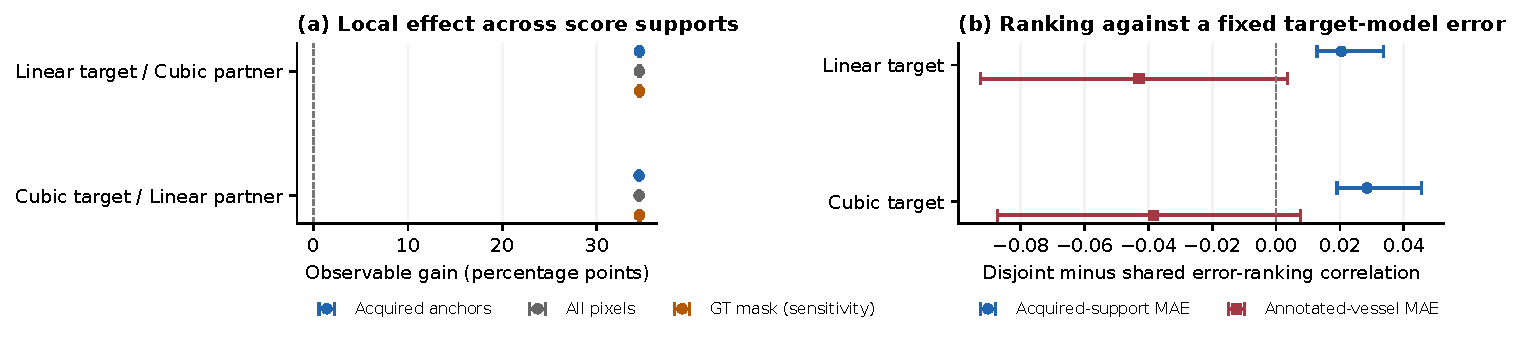
\includegraphics[width=\textwidth]{p14_topcow_external.pdf}
\caption{External MRA local geometry and anatomical ranking. The analytical experiment broadens contrast and endpoint coverage, but does not replicate the five neural models on MRA. Local error exposure is distinct from useful global or vessel-error ordering.}
\end{figure*}

\paragraph{Legacy split and geometry audit.}
The old fastMRI split contains one patient in both train and validation, but test patients overlap neither. Historical checkpoint-selection bias cannot be quantified from the existing outputs. For all 24 paper test cases, original DICOM headers and first/middle/last pixel planes confirm ordering, parallel directions, and monotone physical positions. The stored diagonal NIfTI affine does not retain patient orientation, so agreement of inherited affine matrices alone is insufficient evidence. Source documents in other projects are used for traceability, without importing their developed-model performance as independent evidence.

\paragraph{Anatomical weighting: development and fixed-rule transfer.}
After the TopCoW baseline analysis, we fix a bright-anchor mask at the 95th percentile within each acquired anchor's 1\%-foreground and unite the nearest two masks. The threshold is never searched. TopCoW reuses the development cohort; CAS2023 receives this rule unchanged on all 100 image/label pairs and 6,412 eligible planes. Image and label shapes/affines match. No file hashes match TopCoW, which does not prove person-level nonoverlap without linked identifiers. Unknown CAS header provenance precludes a physical-spacing claim. Cases, residue balancing, estimator rules, and bootstrap count/seed match the preceding protocol.


Before bright weighting, changing shared to disjoint contexts worsens TopCoW vessel-risk coverage: normalized excess risk area increases by .00140 [.00028,.03211] for L and .00135 [.00026,.03120] for C. Full-image score support also yields a negative vessel-ranking change for L, $-.0490$ [$-.1016,-.0003$]. These qualified negative sensitivity results remain part of the evidence.
On TopCoW, all four vessel-risk coverage changes favor bright weighting and all four general-error rankings deteriorate. On CAS2023, the disjoint vessel-risk coverage changes are $-.01047$ [$-.02389,.00034$] and $-.01074$ [$-.02482,.00089$]; shared changes also cross zero. Negative changes in normalized excess risk area favor the new score. Both contexts lose general-error ranking on CAS2023. This is a target-specific ranking transfer with unresolved screening benefit, not a universal score improvement. The full numerical record includes all endpoints and contexts, including nonsignificant and adverse results.


